\documentclass[xcolor={dvipsnames}]{beamer}
\usepackage{color, colortbl}
\usepackage[ngerman,english]{babel}
\usepackage[T1]{fontenc}
\usepackage{CJKutf8} %japanese
\usepackage{lmodern}
\usepackage[compatibility=false]{caption}
\usepackage{subcaption}
\usepackage{tikz}
\usepackage{textgreek}
\usepackage{tabularx}
\usepackage{booktabs}
\usepackage{siunitx}
\usepackage{appendixnumberbeamer}
\usepackage[absolute,overlay]{textpos} %for positioning the logos where I want
\usepackage{xspace,multicol}

\usepackage{animate}
\usepackage{multimedia}

\mode<presentation>
{
  \usetheme{CambridgeUS}     
  \usecolortheme{lily} 
  \definecolor{beamer@violet}{rgb}{0.5,0.3,0.5} % changed this
  \setbeamercolor{structure}{fg=beamer@violet!70!cyan}
  \setbeamercolor{palette primary}{fg=black, bg=gray!30!white!50!cyan!20!}
  \setbeamercolor{palette secondary}{fg=black, bg=gray!30!white!30!cyan!40!}
  \setbeamercolor*{palette tertiary}{bg=gray!20!white!20!cyan!60!}
  
  \setbeamercolor{frametitle}{fg=cyan!60!white!40!,bg=cyan!80!black}
  \setbeamercolor{title}{fg=cyan!80!black}
  \setbeamercolor{normal text}{fg=black,bg=white}
  \setbeamercolor{alerted text}{fg=beamer@violet}
  \setbeamercolor{example text}{fg=beamer@violet!70!cyan}
  
  \usefonttheme{structureitalicserif} 
  \setbeamertemplate{navigation symbols}{}
  \setbeamertemplate{caption}[numbered]
}
\newcommand{\sidlogo}{
  \setlength{\TPHorizModule}{1pt}
  \setlength{\TPVertModule}{1pt}
   % textblock{}{x,y}: pos(x) = rightUpperCorner + (x * \TPHorizModule), pos(y) = leftUpperCorner - (y * \TPVertModule)
  \begin{textblock}{1}(323,12)
   \includegraphics[width=40pt,height=26pt]{figures/SiD.jpeg}
  \end{textblock}
  } 
\newcommand{\ilclogo}{
  \setlength{\TPHorizModule}{1pt}
  \setlength{\TPVertModule}{1pt}
   % textblock{}{x,y}: pos(x) = rightUpperCorner + (x * \TPHorizModule), pos(y) = leftUpperCorner - (y * \TPVertModule)
  \begin{textblock}{1}(323,12)
   \includegraphics[width=40pt,height=26pt]{figures/ILC.jpeg}
  \end{textblock}
} 
\newcommand{\flukalogo}{
  \setlength{\TPHorizModule}{1pt}
  \setlength{\TPVertModule}{1pt}
   % textblock{}{x,y}: pos(x) = rightUpperCorner + (x * \TPHorizModule), pos(y) = leftUpperCorner - (y * \TPVertModule)
  \begin{textblock}{1}(315,12)
   \includegraphics[width=60pt,height=26pt]{figures/fluka_logo.png}
  \end{textblock}
} 
\newcommand{\ejadelogo}{
  \setlength{\TPHorizModule}{1pt}
  \setlength{\TPVertModule}{1pt}
   % textblock{}{x,y}: pos(x) = rightUpperCorner + (x * \TPHorizModule), pos(y) = leftUpperCorner - (y * \TPVertModule)
  \begin{textblock}{1}(323,12)
   \includegraphics[width=40pt,height=26pt]{figures/EJADE.jpeg}
  \end{textblock}
} 
\newcommand{\BDSsymbol}{
  \setlength{\TPHorizModule}{1pt}
  \setlength{\TPVertModule}{1pt}
   % textblock{}{x,y}: pos(x) = rightUpperCorner + (x * \TPHorizModule), pos(y) = leftUpperCorner - (y * \TPVertModule)
  \begin{textblock}{1}(0,39)
   \includegraphics[width=60pt,height=40pt]{figures/Highlight_BDS.png}
  \end{textblock}
} 
\newcommand{\EXTsymbol}{
  \setlength{\TPHorizModule}{1pt}
  \setlength{\TPVertModule}{1pt}
   % textblock{}{x,y}: pos(x) = rightUpperCorner + (x * \TPHorizModule), pos(y) = leftUpperCorner - (y * \TPVertModule)
  \begin{textblock}{1}(0,39)
   \includegraphics[width=60pt,height=40pt]{figures/Highlight_EXT.png}
  \end{textblock}
} 
\newcommand{\ATFlogo}{
  \setlength{\TPHorizModule}{1pt}
  \setlength{\TPVertModule}{1pt}
   % textblock{}{x,y}: pos(x) = rightUpperCorner + (x * \TPHorizModule), pos(y) = leftUpperCorner - (y * \TPVertModule)
  \begin{textblock}{1}(323,12)
   \includegraphics[width=40pt,height=26pt]{figures/ATF_logo.jpg}
  \end{textblock}
} 
\newcommand{\RHULlogo}{
  \setlength{\TPHorizModule}{1pt}
  \setlength{\TPVertModule}{1pt}
   % textblock{}{x,y}: pos(x) = rightUpperCorner + (x * \TPHorizModule), pos(y) = leftUpperCorner - (y * \TPVertModule)
  \begin{textblock}{1}(337,12)
   \includegraphics[width=25pt,height=26pt]{figures/rhul_logo.png}
  \end{textblock}
}

\DeclareSIUnit\year{yr}
\newcommand{\eplus}{e$^+$\xspace}
\newcommand{\eminus}{e$^-$\xspace}


\title[ATF2 Background Simulations]{\textbf{BDSIM simulation model of ATF2 \& Background Studies\\for the Vertical Collimator System}}
\author{\textbf{Anne Sch\"utz}}
\institute{\textbf{KIT, DESY}}
\date{\textbf{April 3, 2017}}

\titlegraphic{
  %\includegraphics[height=1.1cm]{figures/EJADE.png}\hspace*{0.5cm}~%
  \includegraphics[height=1.0cm]{figures/KIT.png}\hspace*{2cm}~%
    \includegraphics[height=1.0cm]{figures/ATF_logo.jpg}\hspace*{3cm}~%
  \includegraphics[height=1.1cm]{figures/DESY_Logo.png}
  %\includegraphics[height=1.0cm]{figures/rhul_logo.png}\hspace*{0.5cm}~%
  %\includegraphics[height=1.0cm]{figures/ific_logo.png}
}

\begin{document}

{
\usebackgroundtemplate{
 \tikz\node[opacity=0.1]{\includegraphics[width=\paperwidth]{figures/Iwatecomics.jpg}};
 % \tikz\node[opacity=0.2]{\centering\includegraphics[height=\paperheight]{figures/Iwatecomics.jpg}};
 }
\begin{frame}
  \titlepage
\end{frame}
}

\begin{frame}{Table of contents}
  \tableofcontents
\end{frame}

%--------------------------------------------------------------

\section{Running BDSIM on the BIRD cluster at DESY}
\begin{frame}
\RHULlogo
Stewart has set up BDSIM at DESY:
\begin{itemize}
 \item locally in my NFS folder
 \item here: (accessable if permissions given)\\
 /afs/desy.de/user/i/iagapov/xxl/mpy/colsim/bdsim-rhul/accsoft/
\end{itemize}
\vspace*{0.2cm}
Use BDSIM by doing:\\
\textcolor{Gray}{\texttt{\small source /etc/profile.d/modules.sh\\                                                
module use {\footnotesize /afs/desy.de/user/i/iagapov/xxl/mpy/colsim/bdsim-rhul/accsoft/modules/all}\\
module load Bdsim\\
source \$EBROOTGEANT4/bin/geant4.sh\\
bdsim --file=atf2.gmad
}}\\
\vspace*{0.2cm}
Submitting jobs to the BIRD cluster for all vertical collimator settings:\\
50 settings, $\sim$ 100 jobs each, 10000 initial particles per job\\
$\rightarrow$ \textit{10000 particles only because BDSIM would enter ``infinite'' loop for very low momentum particles}
\end{frame}





\section{Background studies for the Vertical Collimator System}
\begin{frame}
\ATFlogo
 \begin{center}
    \LARGE Background studies\\for the Vertical Beam Halo Collimator
 \end{center}
\end{frame}

\subsection{Background Measurements at ATF2}
\begin{frame}{The Vertical Beam Halo Collimator and the\\RHUL Cherenkov detector}

\begin{center}
\includegraphics[width=\textwidth]{figures/ATF2schematic.pdf}\\
  \includegraphics[width=\textwidth]{figures/RHUL_detector_Collimator.png}
\end{center}
\end{frame}

\begin{frame}{Background Data taken with the RHUL Cherenkov detector}
\ATFlogo
\begin{center}
 Symmentric jaw movement \hspace*{2.5cm} Jaws moving separately\\
\vspace*{0.2cm}
 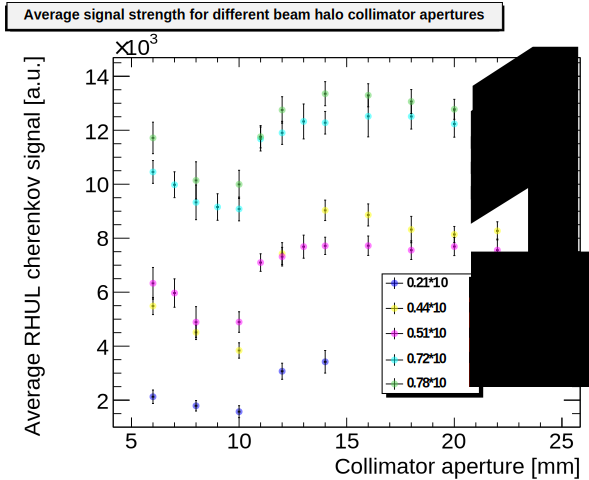
\includegraphics[width=0.55\textwidth]{figures/AverageSignal_perAperture.pdf}
  \includegraphics[width=0.55\textwidth]{figures/AverageSignal_perJawPosition_12April2016.pdf}
\end{center}
Background is reduced, but then rises again when collimator jaws are driven closer into the beam halo.\\
Individual jaw movement gives conflicting results.
%\begin{block}{}
%The vertical beam size at the location of the collimator was about \SI{0.32}{mm} with an offset of 0.2-\SI{0.5}{mm}.
%\end{block}
\end{frame}

\subsection{BDSIM simulation of the Backgrounds at ATF2}
\begin{frame}{Modelling the Vertical Beam Halo Collimator}
\ATFlogo
\begin{center}
View inside the collimator model \hspace*{1cm} Collimator in ATF2 beam line\\
\vspace*{0.2cm}
 \includegraphics[width=0.5\textwidth]{figures/Collimator_model.pdf}
 \includegraphics[width=0.5\textwidth]{figures/Collimator_in_ATF2.png}
\end{center}
The collimator was modelled with \textbf{PyGDML} according to the technical drawings provided by Nuria Fuster Martinez.\\
Its jaws can be placed as desired.
$\Rightarrow$ Individual jaw movement is now possible!
\end{frame}

\begin{frame}{First Data to MC comparison}
\ATFlogo
\begin{center}
\includegraphics[width=0.7\textwidth]{figures/data_mc_comparison.pdf}
\end{center}
First data to MC comparison is not satisfactory.\\
More statistics of the MC is needed, and the ATF2 model in BDSIM needs to be reviewed.
\end{frame}

\begin{frame}{Study of the ATF2 components producing secondary particles}
 \begin{center}
 \only<1>{
\includegraphics[width=0.38\textwidth]{figures/TracksPerModel_firstPart.pdf}
\includegraphics[width=0.38\textwidth]{figures/TracksPerModel_secondPart.pdf}\\
\includegraphics[width=0.38\textwidth]{figures/TracksPerModel_thirdPart.pdf}
\includegraphics[width=0.38\textwidth]{figures/TracksPerModel_forthPart.pdf}\\
Number of particles created in the components of the ATF2 beam line.
}
 \only<2>{
 \begin{columns}
  \begin{column}{0.3\textwidth} 
   \includegraphics[angle=270,width=\textwidth]{figures/ATF2_beamline_firstPart.png}
  \end{column}
 \begin{column}{0.8\textwidth} 
\includegraphics[width=\textwidth]{figures/TracksPerModel_firstPart.pdf}
  \end{column}
 \end{columns}
}
 \only<3>{
  \begin{columns}
  \begin{column}{0.3\textwidth} 
   \includegraphics[angle=270,width=0.7\textwidth]{figures/ATF2_beamline_secondPart.png}
  \end{column}
 \begin{column}{0.8\textwidth}
\includegraphics[width=\textwidth]{figures/TracksPerModel_secondPart.pdf}
  \end{column}
 \end{columns}
}
 \only<4>{
  \begin{columns}
  \begin{column}{0.3\textwidth} 
   \includegraphics[angle=270,width=\textwidth]{figures/ATF2_beamline_thirdPart.png}
  \end{column}
 \begin{column}{0.8\textwidth}
\includegraphics[width=\textwidth]{figures/TracksPerModel_thirdPart.pdf}
  \end{column}
 \end{columns}
}
 \only<5>{
  \begin{columns}
  \begin{column}{0.3\textwidth} 
   \includegraphics[angle=270,width=\textwidth]{figures/ATF2_beamline_forthPart.png}
  \end{column}
 \begin{column}{0.75\textwidth}
\includegraphics[width=\textwidth]{figures/TracksPerModel_forthPart.pdf}
  \end{column}
 \end{columns}
}
\end{center}
\end{frame}

\begin{frame}{Study of the ATF2 components producing secondary particles, sampled in the Vertical Collimator}
These components create particles hitting explicitly the Vertical Collimator:
 \begin{center}
\includegraphics[width=0.6\textwidth]{figures/VertexModels_Comparison_Sampler0.pdf}
\end{center}
\end{frame}
\begin{frame}{Study of the ATF2 components producing secondary particles, sampled in the RHUL detector}
These components create particles hitting the RHUL detector plane:
 \begin{center}
\includegraphics[width=0.6\textwidth]{figures/VertexModels_Comparison_Sampler1.pdf}
\end{center}
\end{frame}
\begin{frame}{Study of the ATF2 components producing secondary particles, sampled in the IP}
These components create particles that reach explicitly the IP:
 \begin{center}
\includegraphics[width=0.6\textwidth]{figures/VertexModels_Comparison_Sampler2.pdf}
\end{center}
\end{frame}

\subsection{Outlook}
\begin{frame}{BDSIM simulation: Outlook}
\ATFlogo
Plans for further BDSIM simulations in collaboration with RHUL:\\
\begin{itemize}
 \item Reviewing the BDSIM geometry model of ATF2
 \item More accurate Aperture Model of ATF2
 \item Put together all new component models for a more accurate ATF geometry model
 \item Improve the Vertical Collimator model
 \item Introduce beam bumps in simulation to study effect of beam orbit changes on background level at the RHUL cherenkov detector and the IP
 \item Change vacuum pressure in the simulation to also compare these data taken
\end{itemize}

\begin{center}
  \includegraphics[width=0.8\textwidth]{figures/atf_bdsim.png}\\
\end{center}

\end{frame}



\section*{The end}
{
\usebackgroundtemplate{
 \tikz\node[opacity=0.1]{\includegraphics[width=\paperwidth,resolution=200]{figures/ilc-Comic.png}};
 % \tikz\node[opacity=0.2]{\centering\includegraphics[height=\paperheight]{figures/Iwatecomics.jpg}};
 }
\begin{frame}
\ATFlogo
\begin{center}
\textcolor{RubineRed}{
	\LARGE Thank you very much!\\
	\vspace*{0.5cm}
	\begin{CJK}{UTF8}{min}
	どうもありがとうございます。
	\end{CJK}
}
\end{center}
\end{frame}
}

\end{document}
